%%
%% This is file `sample-manuscript.tex',
%% generated with the docstrip utility.
%%
%% The original source files were:
%%
%% samples.dtx  (with options: `all,proceedings,bibtex,manuscript')
%% 
%% IMPORTANT NOTICE:
%% 
%% For the copyright see the source file.
%% 
%% Any modified versions of this file must be renamed
%% with new filenames distinct from sample-manuscript.tex.
%% 
%% For distribution of the original source see the terms
%% for copying and modification in the file samples.dtx.
%% 
%% This generated file may be distributed as long as the
%% original source files, as listed above, are part of the
%% same distribution. (The sources need not necessarily be
%% in the same archive or directory.)
%%
%%
%% Commands for TeXCount
%TC:macro \cite [option:text,text]
%TC:macro \citep [option:text,text]
%TC:macro \citet [option:text,text]
%TC:envir table 0 1
%TC:envir table* 0 1
%TC:envir tabular [ignore] word
%TC:envir displaymath 0 word
%TC:envir math 0 word
%TC:envir comment 0 0
%%
%% The first command in your LaTeX source must be the \documentclass
%% command.
%%
%% For submission and review of your manuscript please change the
%% command to \documentclass[manuscript, screen, review]{acmart}.
%%
%% When submitting camera ready or to TAPS, please change the command
%% to \documentclass[sigconf]{acmart} or whichever template is required
%% for your publication.
%%
%%
\documentclass[manuscript,screen,review]{acmart}
%%
%% \BibTeX command to typeset BibTeX logo in the docs
\AtBeginDocument{%
  \providecommand\BibTeX{{%
    Bib\TeX}}}

%% Rights management information.  This information is sent to you
%% when you complete the rights form.  These commands have SAMPLE
%% values in them; it is your responsibility as an author to replace
%% the commands and values with those provided to you when you
%% complete the rights form.
\setcopyright{acmlicensed}
\copyrightyear{2026}
\acmYear{2026}
%\acmDOI{XXXXXXX.XXXXXXX}
%% These commands are for a PROCEEDINGS abstract or paper.
%\acmConference[Conference acronym 'XX]{Make sure to enter the correct
%  conference title from your rights confirmation email}{June 03--05,
%  2018}{Woodstock, NY}
%%
%%  Uncomment \acmBooktitle if the title of the proceedings is different
%%  from ``Proceedings of ...''!
%%
 \acmBooktitle{Computational Imaging and Learning: Practical Approaches to Tomography Data Reconstruction,
   Jun 01, 2026, Padua, IT}
% \acmISBN{978-1-4503-XXXX-X/2026/01}


%%
%% Submission ID.
%% Use this when submitting an article to a sponsored event. You'll
%% receive a unique submission ID from the organizers
%% of the event, and this ID should be used as the parameter to this command.
%%\acmSubmissionID{123-A56-BU3}

%%
%% For managing citations, it is recommended to use bibliography
%% files in BibTeX format.
%%
%% You can then either use BibTeX with the ACM-Reference-Format style,
%% or BibLaTeX with the acmnumeric or acmauthoryear sytles, that include
%% support for advanced citation of software artefact from the
%% biblatex-software package, also separately available on CTAN.
%%
%% Look at the sample-*-biblatex.tex files for templates showcasing
%% the biblatex styles.
%%

%%
%% The majority of ACM publications use numbered citations and
%% references.  The command \citestyle{authoryear} switches to the
%% "author year" style.
%%
%% If you are preparing content for an event
%% sponsored by ACM SIGGRAPH, you must use the "author year" style of
%% citations and references.
%% Uncommenting
%% the next command will enable that style.
%%\citestyle{acmauthoryear}

\input{lstlisting_settings}

\usepackage{fontawesome5}
\usepackage{subcaption}


\definecolor{changes}{HTML}{A42A04}

% Removes ACM stuff
\settopmatter{printacmref=false, printfolios=false}
\renewcommand\footnotetextcopyrightpermission[1]{}
\pagestyle{plain}

\fancypagestyle{firstpagestyle}{
  \fancyhf{}
  \fancyhead[L]{\shortauthors}
  \fancyhead[R]{\thepage}
  \fancyfoot{}  % empty footer, kills "Manuscript submitted to ACM"
}

\AtBeginDocument{
  \fancypagestyle{acmmanuscript}{
    \fancyfoot{}
  }
}
%%
%% end of the preamble, start of the body of the document source.
\begin{document}

%%
%% The "title" command has an optional parameter,
%% allowing the author to define a "short title" to be used in page headers.
\title{Computational Imaging and Learning: Practical Approaches to Tomography Data Reconstruction}

%%
%% The "author" command and its associated commands are used to define
%% the authors and their affiliations.
%% Of note is the shared affiliation of the first two authors, and the
%% "authornote" and "authornotemark" commands
%% used to denote shared contribution to the research.
\author{Marco Bellò}
\email{marco.bello.vi@gmail.com}

%\authornotemark[1]

\affiliation{%
  \institution{University of Padua}
  \city{Padua}
  \country{Italy}
}

%%
%% By default, the full list of authors will be used in the page
%% headers. Often, this list is too long, and will overlap
%% other information printed in the page headers. This command allows
%% the author to define a more concise list
%% of authors' names for this purpose.
\renewcommand{\shortauthors}{Bellò}

%%%%
%%%% The abstract is a short summary of the work to be presented in the
%%%% article.
\begin{abstract}
This report explores the mathematical foundations and practical implementations of Computational Imaging, focusing on two complementary inverse problems: Image Scanning Microscopy (ISM) and Computed Tomography (CT). The shared common structure is that an unknown spatial distribution must be recovered from indirect, noisy measurements through a linear forward operator. Starting from the physical principles underlying each modality, the report derives the forward model and frames reconstruction as an ill-posed inverse problem requiring regularisation. For CT, a series of model-based reconstruction algorithms are implemented using the DeepInverse library, from Filtered Back-Projection through Tikhonov and LASSO regularisation, to trained Plug-and-Play DnCNN denoising priors. Results demonstrate that training a task-specific denoiser outperforms both classical methods and denoisers pretrained on natural images, underscoring the importance of domain-appropriate priors.
\end{abstract}
%%
%%
%%%%
%%%% The code below is generated by the tool at http://dl.acm.org/ccs.cfm.
%%%% Please copy and paste the code instead of the example below.
%%%%



%%%%
%%%% Keywords. The author(s) should pick words that accurately describe
%%%% the work being presented. Separate the keywords with commas.
\keywords{computed tomography, image scanning microscopy}
%%
\received{01/06/2026}
%\received[revised]{27/05/2026}
%%\received[accepted]{24/19/2025}

%%
%% This command processes the author and affiliation and title
%% information and builds the first part of the formatted document.
\maketitle
% removes footer "Manuscript submitted to ACM"
\thispagestyle{plain}  % fixes page 1
\pagestyle{plain}


%\section{Introduction and Mathematical Foundations}
In traditional photography, image acquisition is a direct process: a physical lens focuses light reflected from an object onto a photosensitive sensor, comprised by billions of photosites each of which records the raw intensity values of light in three channels: Red, Green, and Blue. The post-processing needed to then obtain a polished-looking picture are quite straightforward, since the object of interest is the \textit{external} appearance of the subject.

On the other hand, many modern scientific and medical apparatuses require looking inside an object to capture phenomena where direct visual access is not possibile, for example when taking an X-Ray of a patient. In this paradigm, the raw hardware measurements are often highly degraded, indirect, or completely unrecognizable, and the final image must be computationally reconstructed. This constraint gave rise to the interdisciplinary field of \textit{Computational Imaging} (CI), which leverages machine learning and other paradigms to overcome hardware limitations and reconstruct high-quality images from raw, unstructured sensor data. This represents a paradigm shift in visual and diagnostic modalities, transitioning to an integrated approach that couples physical measurement devices with rigorous data-driven and variational algorithms.

An example of an application of computational imaging is MRI subsampling: the idea is to purposely acquire only a fraction of the raw data to speed-up the process of a factor of 2X to 10X, to minimize claustrophobia in patients. The image is then reconstructed from the incomplete data.

\subsection{The Continuous Forward Physics Model}
The fundamental starting point for any analytical treatment of an imaging system is the establishment of a forward model. Let $u \in \mathcal{U}(\mathbb{R}^d)$ represent the continuous, unknown physical object of interest embedded in a $d$-dimensional space. The process of signal transmission and subsequent digital recording can be encapsulated by the generic continuous-to-discrete forward operator mapping defined as:
\begin{equation}
    y = \mathcal{P}(\mathcal{S}\mathcal{H}u)
\end{equation}
where $y \in \mathbb{R}^M$ denotes the vector of $M$ discrete, experimental observations. The linear operators perform distinct tasks mandated by the physical architecture of the scanning device:
\begin{itemize}
    \item $\mathcal{H}: \mathcal{U}(\mathbb{R}^d) \to \mathcal{Y}(\mathbb{R}^{d_0})$ maps the continuous object space to a continuous signal space via a linear integral operator governed by a physical kernel $h(z,x)$:
    \begin{equation}
        (\mathcal{H}u)(z) = \int_{\mathbb{R}^d} h(z, x) u(x) \, dx
    \end{equation}
    Depending on the modality, this kernel models phenomena such as pointwise multiplication, shift-invariant blurs ($h(z,x) = k(x-z)$), or line-integral projections.
    \item $\mathcal{S}: \mathcal{Y}(\mathbb{R}^{d_0}) \to \mathbb{R}^M$ is a localized sampling operator that models detector boundaries and pixel/voxel integration arrays using sampling weights $\psi_m(z)$:
    \begin{equation}
        [\mathcal{S}v]_m = \int_{\mathbb{R}^{d_0}} \psi_m(z) v(z) \, dz, \quad \forall m \in \{1, \dots, M\}
    \end{equation}
    \item $\mathcal{P}: \mathbb{R}^M \to \mathbb{R}^M$ characteristically models stochastic structural degradations, such as electronic read noise or quantum photon counting restrictions.
\end{itemize}

\subsection{Finite-Dimensional Discretization and Matrix Structures}
Because digital computing systems cannot directly process infinite-dimensional continuous spaces, we must approximate the continuous operator by projecting $u$ onto an $N$-dimensional approximation space $\mathcal{U}_N(\mathbb{R}^d) = \text{span}(\{\phi_n\}_{n=1}^N)$ comprised of linearly independent generating functions or basis elements (e.g., splines, wavelets, or indicator functions on a localized pixel grid)~. Writing $u \approx \sum_{n=1}^N u_n \phi_n$ allows the linear system to be expressed through a matrix-vector product:
\begin{equation}
    \mathcal{S}\mathcal{H}u \approx A_0 u
\end{equation}
where $A_0 \in \mathbb{R}^{M \times N}$ represents the discrete forward operator matrix given by the exact integral evaluation $[A_0]_{m,n} = [\mathcal{S}\mathcal{H}\phi_n]_m$. 

For realistic scales (e.g., $M = N = 10^7$), constructing and storing $A_0$ explicitly poses catastrophic memory requirements ($\approx 800$ Terabytes) and computationally prohibitive matrix multiplications ($O(MN)$). Computational imaging therefore leverages highly structured linear approximations, relying on numerical integration quadrature rules ($\hat{A}$) and structural sparsification thresholds ($A = \mathcal{T}(\hat{A})$). Depending on the specific physical geometry, the system can be approximated via $K$-sparse matrices under Compressed Sparse Row (CSR) storage schemes, multi-diagonal band structures for decaying spatial kernels, circulant structures diagonalizable via Fast Fourier Transforms ($A = \mathcal{F}^{-1} \text{diag}(\mathcal{F}c)\mathcal{F}$), or low-rank singular value compositions.

\subsection{Ill-Posedness and Inversion Failure}
A fundamental challenge in solving the inverse problem—recovering the vector $u \in \mathbb{R}^N$ from the corrupted observations $y \in \mathbb{R}^M$—is the inherent ill-posedness of the system in the sense of Hadamard. A problem is considered well-conditioned if a solution exists within the image space, is strictly unique, and exhibits topological stability such that localized modifications in the data vector do not produce unbounded variations in the reconstruction. 

In practical implementations, the measurement vector is perturbed by additive white noise, $y = Au + n$, where $n \sim \mathcal{N}(0, \sigma^2 I_M)$. Standard direct algebraic inversions fail completely in this setting. If one attempts a naive direct matrix inversion or a standard least-squares minimization:
\begin{equation}
    u_{LS} \in \arg\min_{u \in \mathbb{R}^N} \frac{1}{2} \|Au - y\|_2^2
\end{equation}
the presence of zero or near-zero singular values within the spectrum of $A$ catastrophically amplifies the noise component. Evaluating the stable minimum-norm solution via the Moore-Penrose pseudo-inverse $A^{\dagger} = V \Sigma^{-1} U^T$ reveals the nature of this structural instability:
\begin{equation}
    u^* = A^{\dagger}y = \bar{u} + V \Sigma^{-1} U^T n
    \label{eq:pseudoinverse}
\end{equation}
The relative error is bounded by the condition number $\kappa(A) = \sigma_1(A) / \sigma_R(A)$. As the singular values $\sigma_R(A)$ decay precipitously toward zero, $\kappa(A) \to \infty$, causing the noise term in Equation \eqref{eq:pseudoinverse} to dominate the signal entirely and rendering the reconstructed image useless.

\subsection{Variational Regularization Frameworks}
To stabilize this inversion, it is mandatory to incorporate a priori architectural assumptions regarding the expected structural properties of the target image. This is formalized mathematically through a variational minimization problem balancing a data fidelity term and a regularizing constraint:
\begin{equation}
    u^* \in \arg\min_{u \in \mathbb{R}^N} \mathcal{D}(Au, y) + \lambda \mathcal{R}(u)
\end{equation}
Here, $\mathcal{D}(\cdot,\cdot)$ ensures physical compliance with the measured values, derived from statistical likelihood specifications via a Bayesian paradigm (e.g., quadratic $\frac{1}{2}\|Au-y\|_2^2$ fields under Gaussian perturbations, or Kullback-Leibler divergences under Poisson particle dynamics). The parameter $\lambda > 0$ dictates the optimization trade-off between experimental measurements and spatial expectations. 

The chosen image model $\mathcal{R}(u)$ completely shapes the geometry of the solution space. Basic energy minimization ($\mathcal{R}(u) = \|u\|_2^2$) stabilizes numerical conditioning but lacks local feature preservation. Standard Tikhonov-Sobolev smoothness regularizers ($\mathcal{R}(u) = \|\nabla u\|_2^2$) enforce global derivative penalties that penalize oscillations, yet systematically blur highly localized structural bounds and crisp target edges. To overcome this oversmoothing, edge-preserving alternatives such as Total Variation ($\text{TV}(u) = \sum_n \|\nabla u[n]\|_2$) are implemented to foster sparse gradient fields, creating piecewise-constant block representations. Alternatively, sparse representation approaches project the candidate image onto directional frame dictionaries ($\Psi$) under localized $\ell_1$-norm penalties ($\| \alpha \|_1$), utilizing convex optimization proxies to resolve complex underlying physical parameters.

\subsection{Transition to Section 2: Computed Tomography}
While standard architectural variations—such as shift-invariant blurs or uniform spatial degradations—provide excellent intuitive templates for variational design, they do not fully reveal the mathematical complexity encountered when the operator $A$ maps completely separate physical spaces. To fully analyze the performance of these analytical tools, we must examine a medical modality where the measurement space is inherently non-local and fundamentally decoupled from the classical spatial coordinate framework: \textbf{Computed Tomography (CT)}. 

As outlined in the next section, the physics of X-ray attenuation transitions the forward operator from a local localized transformation into a series of boundary line integrals formalized by the continuous X-ray and Radon transforms. Resolving this specific modality demands an explicit study of projection geometries, sinogram spaces, and customized optimization architectures designed to invert non-local physical operators without introducing severe noise amplification or structural artifacts.

\section{Introduction}

In traditional photography, image acquisition is a direct process: a physical lens focuses light reflected from an object onto a photosensitive sensor, comprised by billions of photosites each of which records the raw intensity values of light in three channels: Red, Green, and Blue. The post-processing needed to then obtain a polished-looking picture are quite straightforward, since the object of interest is the \textit{external} appearance of the subject.

On the other hand, many modern scientific and medical apparatuses require looking inside an object to capture phenomena where direct visual access is not possibile, for example when taking an X-Ray of a patient. In this paradigm, the raw hardware measurements are often highly degraded, indirect, or completely unrecognizable, and the final image must be computationally reconstructed. This constraint gave rise to the interdisciplinary field of \textit{Computational Imaging} (CI), which leverages machine learning and other paradigms to overcome hardware limitations and reconstruct high-quality images from raw, unstructured sensor data. This represents a paradigm shift in visual and diagnostic modalities, transitioning to an integrated approach that couples physical measurement devices with rigorous data-driven and variational algorithms.

An example of an application of computational imaging is MRI undersampling: the idea is to purposely acquire only a fraction of the raw data to speed-up the process of a factor of 2X to 10X, to minimize claustrophobia in patients. The image is then reconstructed from the incomplete data.

Mathematically, the core of Computational Imaging lies in the distinction between the \textit{forward problem} and the \textit{inverse problem}. The forward problem models the underlying physics of the imaging system. Assuming the true, continuous underlying object is represented by $u$, and the discrete, noisy measurements recorded by the hardware are $y$, the acquisition process can be formulated as:
\begin{equation}
    y = Au + \eta
\end{equation}
where $A$ represents the forward operator (e.g., a blurring kernel, a Fourier transform, or a Radon transform) dictated by the system's physics, and $\eta$ denotes noise added by the measurement. The objective of Computational Imaging is to solve the corresponding \textit{inverse problem}: given the corrupted measurements $y$ and the known or estimated forward operator $A$, find an approximation $u'$ that accurately recovers the true state of the object.

Two concrete and complementary archetypes of such inverse problems are explored in this essay. The first is \textit{Image Scanning Microscopy} (ISM), a fluorescence imaging modality in which a two-dimensional detector array replaces the single-element detector of a confocal microscope, yielding a four-dimensional dataset. Here the forward operator is a convolution with a Point Spread Function (PSF), and the reconstruction task consists of recovering a fluorophore map from multiple noisy and shifted views of the same subject. The second is \textit{Computed Tomography} (CT), where a scanner measures the attenuation of X-ray beams passing through the body at various angles, producing raw data known as a sinogram. In this case the forward operator is the Radon transform, and the reconstruction task is to recover a cross-sectional image from a series of indirect projections. Despite their different physical origins and scales, both problems are governed by the same mathematical structure: a linear forward operator whose inversion is ill-posed, requiring principled regularisation or learned priors to yield stable and high-quality reconstructions.

The last half of this essay explores practical approaches to Computed Tomography, implemented using the \textit{DeepInverse} library. First, we will reconstruct a precise internal cross-sections, with the raw data represented as a sonogram, consisting of discrete, noisy line integrals corrupted by noise.  The objective is to formulate a rigorous forward model of the scanning process based on the discrete Radon transform and solve the resulting ill-posed inverse problem to recover the tissue attenuation map. We will implement optimization algorithms for Maximum Likelihood and Maximum a Posteriori estimation.

Then, we will try to learn the prior distribution implicitly from data. We will explore \textit{Plug-and-Play (PnP) Priors}, replacing the proximal operator of the regularizer with a pre-trained deep denoising neural network. This is a hybrid approach that combines known physics with learned image statistics. Lastly, we will train our own denoiser to use it in a PGD network.

\paragraph{Sources}

The main sources for this essay are the following:

\begin{itemize}
    \item Prof. Luca Calatroni's mini-course slides "Computational imaging \& learning: from physics to data-driven methods";
    \item C. A. Bouman, Foundations of Computational Imaging: A Model-Based Approach, SIAM, 2022 \cite{bouman_foundations_2022};
    \item G. Aubert, P. Kornprobst, Mathematical Problems in Image Processing: PDEs and the COV, II edition, Springer, 2000 \cite{aubert_mathematical_2008};
    \item Tony F. Chan, J. Shen, Image Processing and Analysis: variational, PDE, wavelet and stochastic methods, SIAM, 2005 \cite{chan_image_2005};
    \item Tristan van Leeuwen's blog \cite{van_leeuwen_1_nodate};
    \item Johannes Meyer's blog \cite{meyer_computational_nodate};
    \item Numerical tours by G. Peyré \cite{peyre_numerical_nodate};
    \item DeepInverse tutorials \cite{deepinverse_examples_nodate}.
\end{itemize}

\section{Image Scanning Microscopy}

Modern biological and biomedical research frequently demands the ability to image
microscopical structures, from one micrometer bacteria to amino acids in the nanometer scale. Optical microscopy has long been
the workhorse of such investigations, owing to its non-invasive nature and compatibility
with live specimens. Yet imaging at this scale is far from straightforward: two
fundamental requirements, \textit{high contrast} and \textit{high resolution}, are
each difficult to achieve and often stand in tension with one another. Moreover, conventional microscopy falls short under the micrometer scale, thus being incapable of observing structures such as viruses or proteins.

\subsection{Fluorescence Microscopy and the Diffraction Limit}

Fluorescence microscopy addresses the contrast challenge by exploiting the phenomenon of fluorescence: certain molecules (fluorophores) absorb excitation light at a shorter wavelength and re-emit it at a longer, less energetic wavelength. By selectively labelling specific cellular structures with fluorescent markers, one can visualize components of interest against a dark background with high specificity, effectively filtering out the rest of the sample. A widefield fluorescence microscope routes a laser excitation beam through an objective lens onto the specimen; the emitted fluorescent light is then separated from the excitation by a dichroic mirror and emission filter, and collected by a detector to form an image.

Resolution, however, is fundamentally bounded by the wave nature of light. A lens cannot focus an electromagnetic beam to an infinitely small spot. Instead, each point in the sample is imaged as a diffuse blob known as the \textit{Point Spread Function} (PSF). The width of the PSF determines the smallest resolvable feature: two emitters closer together than the PSF width are indistinguishable. This is formalized by the \textit{Abbe diffraction limit}, which states that the minimal resolvable distance $d$ satisfies
\begin{equation}
    d = \frac{\lambda}{2 \, \mathrm{NA}} = \frac{\lambda}{2 n \sin(\theta)}
    \approx 200\text{--}250 \; \text{nm},
\end{equation}
where $\lambda$ is the emission wavelength, $\mathrm{NA}$ is the numerical aperture of the objective, $n$ is the refractive index of the immersion medium, and $\theta$ is the half the angle of the acceptance cone. 

Equivalently, in the frequency domain, the \textit{Optical Transfer Function} (OTF) acts as a low-pass filter, suppressing spatial frequencies beyond a cutoff determined by the numerical aperture.

The consequence is that widefield fluorescence microscopy is limited to observe a surface of roughly a quarter of a micrometer, translating in the need of image reconstruction pipelines.

\subsection{Confocal Laser Scanning Microscopy}

The \textit{Confocal Laser Scanning Microscope} (CLSM) improves upon widefield imaging by replacing camera-based wide-area detection with a point-by-point scanning strategy. A focused laser beam is raster-scanned across the specimen using galvanometric mirrors; at each scan position $\mathbf{x}_s$, the emitted fluorescence passes back through the objective and is focused through a small \textit{pinhole} aperture onto a detector (for example a photodiode), which records a single photon-count value. The pinhole rejects anything that os out of focus, which has two advantages: optical sectioning (the ability to reconstruct thin focal planes within a thick specimen) and, when the pinhole is closed down, a modest improvement in lateral resolution beyond the Abbe limit by up to a factor of $\sqrt{2}$.

These gains come at a cost. Closing the pinhole necessarily discards a large fraction of the collected photons, severely reducing the signal-to-noise ratio (SNR), which leads to a situation that is never optimal: a wide pinhole recovers photon counts but degrades both sectioning and resolution, while a narrow pinhole improves spatial quality at the expense of a dim, noisy image. 

\subsection{Image Scanning Microscopy: Concept and Data Structure}

\textit{Image Scanning Microscopy} (ISM) resolves the CLSM trade-off by replacing the single-element detector with a two-dimensional \textit{Single-Photon Avalanche Diode (SPAD) array}. The array, approximately $1.4$ Airy Units, is centred on the optical axis. For each scan position $\mathbf{x}_s = (x_s, y_s)$, rather than integrating all arriving photons into one number, every pixel $\mathbf{x}_d = (x_d, y_d)$ of the detector array records its own photon count independently. A complete ISM acquisition therefore produces a \textit{four-dimensional dataset} $i(\mathbf{x}_s \mid \mathbf{x}_d)$, consisting of $(N_x \times N_y)$ micro-images (one per scan point), each of which is a small image of the sample as seen by a particular detector element. Equivalently, one may reorganize the same data as $N_\mathrm{ch}$ scanned images (one per detector pixel). This high-dimensional dataset carries substantially more spatial information than a conventional confocal acquisition and is a defining feature of the ISM modality \cite{zunino_open-source_2023}.

\subsection{Forward Model and the Inverse Problem}

The image formation process in fluorescence microscopy is well described as a \textit{linear shift-invariant} (LSI) system. The observed image is the convolution of the unknown fluorophore distribution $\mathbf{u} \in \mathbb{R}^N_+$ with the system's PSF $h$, corrupted by Poisson noise $\mathcal{P}$: 
\begin{equation} 
    \mathbf{y} = \mathcal{P}(\mathbf{h} * \mathbf{u}) = \mathcal{P}(\mathbf{A}\mathbf{u}), 
\end{equation} where $\mathbf{A} \in \mathbb{R}^{N \times N}$ is the Toeplitz matrix computing the convolution with the PSF. In CLSM the PSF is a product of the excitation PSF and the effective detection PSF shaped by the pinhole. 

In the ISM setting, the forward model generalizes to a family of $d$ equations 
\begin{equation} 
    \mathbf{y}_d = \mathcal{P}(\mathbf{h}_d * \mathbf{u}) = \mathcal{P}(\mathbf{A}_d \mathbf{u}), \qquad d = 1, \ldots, 25, 
\end{equation} 
where $\mathbf{y}_d \in \mathbb{N}^N$ is the measured image from detector $d$ with $p = n_1 \times n_2$ pixels, $\mathbf{u} \in \mathbb{R}_+^N$ is the unknown object, $\mathbf{A}_d \in \mathbb{R}^{N \times N}$ is the Toeplitz matrix to compute the convolution with the PSF $h_d$, and $\mathcal{P}$ is the Poisson noise.

Optical aberrations such as spherical aberration, astigmatism, and coma are common sources of PSF distortion in fluorescence microscopy, arising from refractive index mismatches, intentional depth encoding, or element misalignment. As illustrated by figure \ref{fig:ismexamples}, these aberrations manifest as characteristic deformations in both the detector offset patterns and the reconstructed PSF shapes, degrading spatial resolution and image quality. Accurately modeling and correcting for these effects is therefore essential for reliable reconstruction in any computational microscopy pipeline.

\begin{figure}[h]
  \centering
  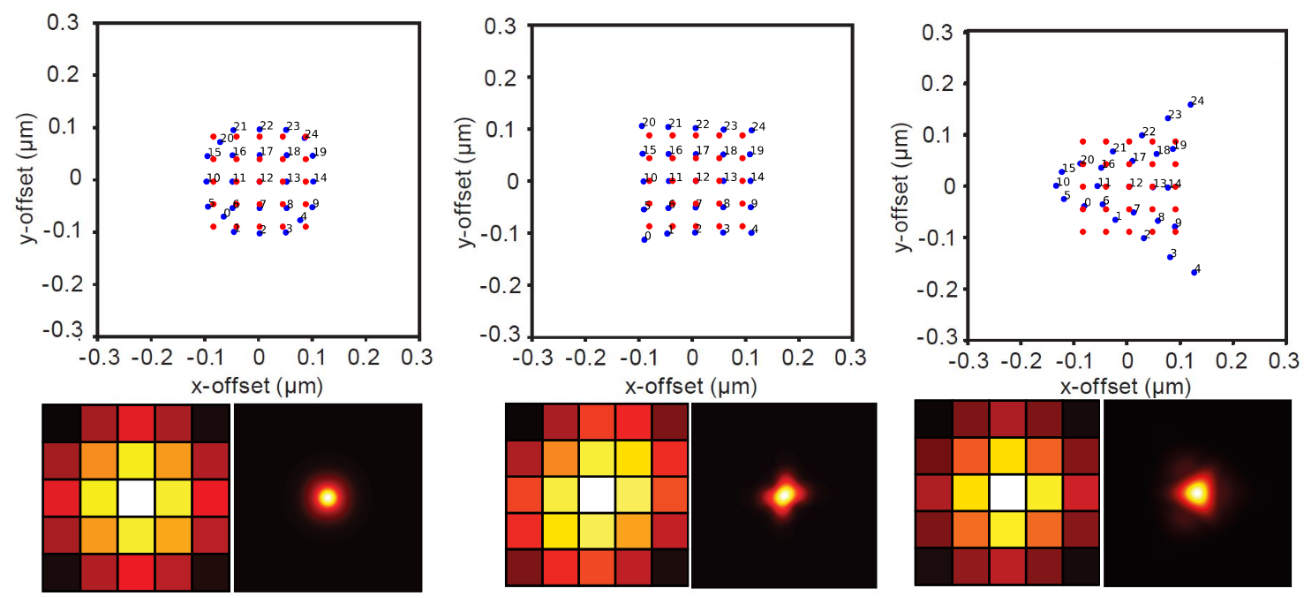
\includegraphics[width=.8\linewidth]{images/ismexamples.png}
  \caption{Aberrations examples on ISM.}
  \label{fig:ismexamples}
\end{figure}

\subsection{From Microscopy to Tomography}

The inverse problem structure of ISM shares mathematical parallels with that of Computed Tomography, discussed in the following section. In both cases, the objective is to recover an unknown spatial distribution from a collection of indirect, noisy measurements related to it through a linear forward operator. In ISM the forward operator is a convolution (a consequence of the LSI imaging model), while in CT it is the Radon transform (a consequence of straight-line X-ray propagation). Both are compact linear operators whose inversion is ill-posed and requires regularisation. Moreover, just as ISM acquires multiple shifted views of the same object, CT acquires projections from multiple angles with each angular view illuminating a different set of line integrals through the target. 

Both settings exemplify the broader programme of computational imaging, in which the design of the acquisition, the modelling of the forward physics, and the inversion algorithm are optimized to extract the maximum information about an object from measurements that are always finite, incomplete, and noisy.

\paragraph{Sources}

The list of sources for this section follow:
\begin{itemize}
    \item Slides \textit{"Image Scanning Microscopy: from forward to inverse problem formulations"}, authored by Luca Calatroni, Lisa Cuneo, and Giuseppe Vicidomini;
    \item A. Zunino et al., "Open-source tools enable accessible and advanced image scanning microscopy data analysis", Nature Photonics volume 17, pp 457–458 (2023) \cite{zunino_open-source_2023};
    \item A. Zunino et al., "Structured detection for simultaneous super-resolution and optical sectioning in laser scanning microscopy", Nature Photonics volume 19, pp 888–897 (2025) \cite{zunino_structured_2025};
    \item B. Richard and E. Wolf, Electromagnetic diffraction in optical systems II, Proceedings of the Royal Society of London. A. Mathematical and Physical Sciences (1959) \cite{richards_electromagnetic_1959};
    \item Y. Liu, V. Stergiopoulou et al, "Revisiting PSF models: unifying framework and high-performance implementation", arxiv DOI, (2025) \cite{liu_revisiting_2025};
    \item F. Fersini et al, Wavefront estimation through structured detection in laser scanning microscopy, Biomed. Opt. Express (2025) \cite{fersini_wavefront_2025}.
\end{itemize}

\section{Computed Tomography}

Computed Tomography (CT) is a non-invasive imaging technique that reconstructs the internal structure of an object from measurements taken externally. The term \textit{tomography} itself derives from the Greek words \textit{tomos} (slice or section) and \textit{graphein} (to write or record), which reflect its purpose of producing representations of a target by observing cross-sectional images of a target without physical intervention.

The physical principle underlying Computed Tomography relies on the transmission of waves or particles, most commonly X-rays, through the object of interest. As X-rays traverse matter, their intensity is attenuated according to the material's local properties. In the simplest homogeneous case, this relationship is captured by the exponential decay $I_1 = I_0 e^{-\mu s}$, where $I_0$ and $I_1$ denote the incident and transmitted intensities, $\mu > 0$ is the attenuation coefficient, and $s$ is the path length through the material. For non-homogeneous objects, this generalizes to $I_1 = I_0 \, e^{-\int_{\ell} \mu(x)\, dx}$. The \textit{Beer-Lambert law} can be used to connect the the initial and final intensities of an X-ray:

\begin{equation}
    I_1 = I_0 \, e^{-\int_{\ell} \mu(x)\, dx} \Longleftrightarrow -\log(I_1/I_0) = \int_{\ell} \mu(x)\, dx
\end{equation} 

As a result, during a tomographic scan, $I_0$ is known from calibration and $I_1$ from measurements. $I_1$ is measured along many lines $\ell_{(\omega,s)}$ to get many line integral values through the object. The intensity $I_1$ is called the \textit{transmission}, while the corresponding $-\log(I_1/I_0)$ is called absorption or \textit{projection}, and a collection of projections is called a \textit{sinogram}.

Mathematically, CT reconstruction can be cast as an inverse problem. Given a target $u \in X = L^2(\Omega)$ with $u \colon \mathbb{R}^d \to \mathbb{R}_+$ defined on a bounded domain $\Omega \subset \mathbb{R}^d$ ($d = 2, 3$), the \textit{forward problem} models the acquisition process via the Radon transform $\mathcal{R}(u) = y$, which integrates $u$ over lines $\ell(\omega, s)$ parameterized by $(\omega,s) \in S^1 \times \mathbb{R}$. The reconstruction task, i.e., recovering $u$ from measured data $y$, constitutes the corresponding \textit{inverse problem}.

The classical analytic solution to this inverse problem is \textit{Filtered Backprojection} (FBP), an exact inversion formula valid in the continuous setting. FBP performs well when complete projection data are available and the target can be assumed static. However, it suffers from theoretical limitations under discretization and provides no stability guarantees in realistic acquisition conditions.

In many practical scenarios, reducing the X-ray radiation dose or shortening scan time leads to \textit{limited data tomography}, which encompasses two main regimes: \textit{limited-angle CT}, where projections are acquired only within a restricted angular range, and \textit{sparse-angle CT}, where a reduced number of projection angles are sampled over the full range. Both settings cause FBP to produce severely degraded reconstructions, motivating the development of more advanced reconstruction methods capable of handling incomplete and noisy measurement data. Both scenarios can be seen in figure \ref{fig:fbprobe}.

\begin{figure}[h]
    \centering
    \begin{minipage}{0.8\linewidth}
        \centering
        \begin{subfigure}{0.49\textwidth}
            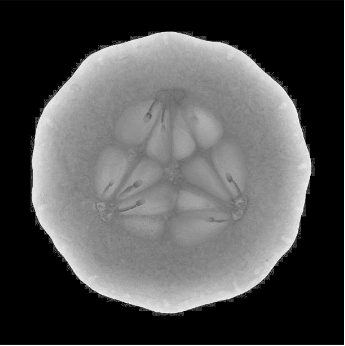
\includegraphics[width=\linewidth]{images/ctground.png}
            \caption{Ground truth}
        \end{subfigure}
        \hfill
        \begin{subfigure}{0.49\textwidth}
            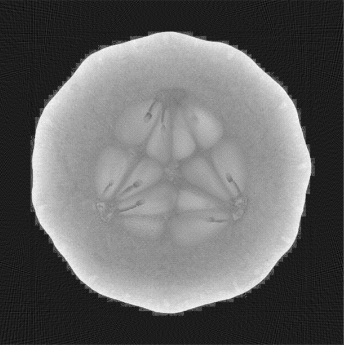
\includegraphics[width=\linewidth]{images/ctfullangle.png}
            \caption{FBP from full angle data}
        \end{subfigure}

        \vspace{0.5em}

        \begin{subfigure}{0.49\textwidth}
            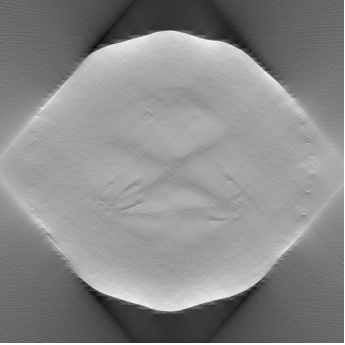
\includegraphics[width=\linewidth]{images/ctlimitedangle.png}
            \caption{FBP from limited-angle data}
        \end{subfigure}
        \hfill
        \begin{subfigure}{0.49\textwidth}
            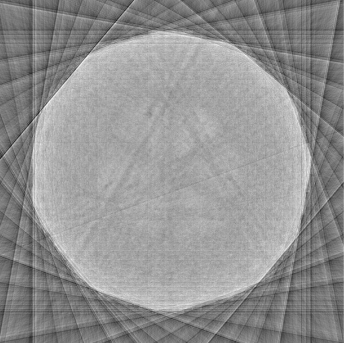
\includegraphics[width=\linewidth]{images/ctsparseangle.png}
            \caption{FBP from sparse angle data}
        \end{subfigure}

        \caption{Limited data tomography: examples.}
        \label{fig:fbprobe}
    \end{minipage}
\end{figure}

\section{Simulating and Reconstructing Tomography Data}

In this last section, we will go trough a series of practical experiments to, using the \textit{DeepInverse} library, to simulate and reconstruct tomography data.

The source code for this section can be seen in the Jupyter noteebok at the following link: \href{https://github.com/mhetacc/CIL/blob/6830cc50b972bd39f5c5c328295af87e33732a38/notebooks/CompleteCTlab.ipynb}{github/mhetacc/.../CT.ipynb}

\subsection{Model-Based Reconstruction}

The first objective is recovering an image $u$ from a set of noisy projections $y$. The measurements are modelled via the \textit{discrete Radon transform}
\begin{equation}
    \begin{aligned} \mathbf{y}(\boldsymbol{\theta},\rho) &= \int_{L_{\boldsymbol{\theta},\rho}}~u~d\sigma
    \end{aligned} \qquad \boldsymbol{\theta} \in \mathbb{R}^2,~ \| \boldsymbol{\theta}\|=1, \quad \rho \in \mathbb{R}_+
\end{equation}
where the collection of projections across all angles is called the \textit{sinogram}. 

Three acquisition geometries are studied: (i) \textit{full-angle} (180 projections), (ii) \textit{sparse-angle} (36 uniformly sampled angles), and (iii) \textit{limited-angle} (between 30 and 150 degrees). An example of the code for the definition of the forward model with 36 angles is shown in listing \ref{code:forward}.

\begin{lstlisting}[language=Python, label={code:forward}, caption={Defining the sparse-angle CT forward model with \textit{deepinv}.}]
import deepinv as dinv
import torch

theta_sparse = torch.tensor(
    np.linspace(0, 180, 36, endpoint=False)
).to(device)

tomo_sparse = dinv.physics.Tomography(
    angles=theta_sparse,
    img_width=128,
    circle=False,
    device=device
)

sinogram_sparse = tomo_sparse(u_SL_small)
\end{lstlisting}

Resulting sinograms can be seen in figure \ref{fig:sinograms}.

\begin{figure}[h]
    \centering
    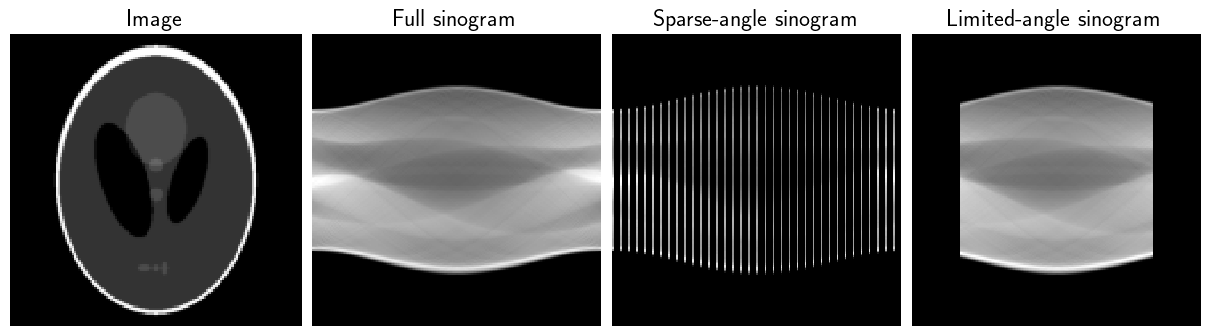
\includegraphics[width=.8\linewidth]{images/sinograms.png}
    \caption{Original image (on the left) and its sinograms under full-angle, sparse-angle, and limited-angle geometries.}
    \label{fig:sinograms}
\end{figure}

Gaussian noise is added to the sinogram via a custom class that scales the noise amplitude by $\max|x|$, making it signal-dependent (Listing~\ref{code:noise}).

\begin{lstlisting}[language=Python, label={code:noise}, caption={Custom Gaussian noise model for CT sinograms.}]
class GaussianNoiseCT(dinv.physics.GaussianNoise):
    def forward(self, x, sigma=None, seed=None, **kwargs):
        self.update_parameters(sigma=sigma, **kwargs)
        self.to(x.device)
        return (x + torch.max(torch.abs(x))
                * self.randn_like(x, seed=seed)
                * self.sigma[(...,) + (None,) * (x.dim()-1)])
\end{lstlisting}

\subsubsection{Näive inversion: Filtered Back-Projection}

An inverse problem can be representing as recovering $f$ from
$y = \text{noise}(A(u))$. When $A$ is linear, in the discrete formulation, this reduces to
\begin{equation}
    y = \mathbf{A} u + \epsilon, \quad u \in \mathbb{R}^n, \epsilon \in \mathbb{R}^m, \mathbf{A} \in \mathbb{R}^{m \times n}
\end{equation}

The simplest reconstruction strategy is to use \textit{Filtered Back-Projection} (FBP) to solve $u_{\text{naive}} = \mathbf{A}^{-1} y$. It is available directly from the physics object via \textit{tomo.fbp(sinogram)}. While fast, FBP is highly sensitive to noise and to incomplete angular coverage.

\subsubsection{Gradient Descent (unregularized)}

To avoid assembling the dense matrix $\mathbf{A}$, iterative solvers minimize $\frac{1}{2}\|\mathbf{A}u - y\|^2$ via gradient descent:
\begin{equation}
    \left\{
    \begin{aligned}
    u^{0} & \text{ given} \\
    u^{(k+1)} =&\  \mathbf{A}^T(\mathbf{A}u^{(k)}-y)
    \end{aligned}
    \right.
\end{equation}

In \textit{deepinv} this is assembled with \textit{optim\_builder} using a \textit{ZeroPrior} (example in listing \ref{code:gd}).

\begin{lstlisting}[language=Python, label={code:gd}, caption={Unregularised gradient descent reconstruction.}]
prior = dinv.optim.prior.ZeroPrior()

opt = dinv.optim.optim_builder(
    iteration="GD",
    prior=dinv.optim.prior.ZeroPrior(),
    data_fidelity=dinv.optim.data_fidelity.L2(),
    max_iter=100,
    crit_conv="residual",
    thres_conv=1e-4,
    early_stop=True,
    params_algo={"stepsize": 1.0}
)
u_hat, metrics = opt(y, tomo_exp, compute_metrics=True)
\end{lstlisting}

Results can be seen in figure \ref{fig:gradescent}.

\begin{figure}[h]
    \centering
    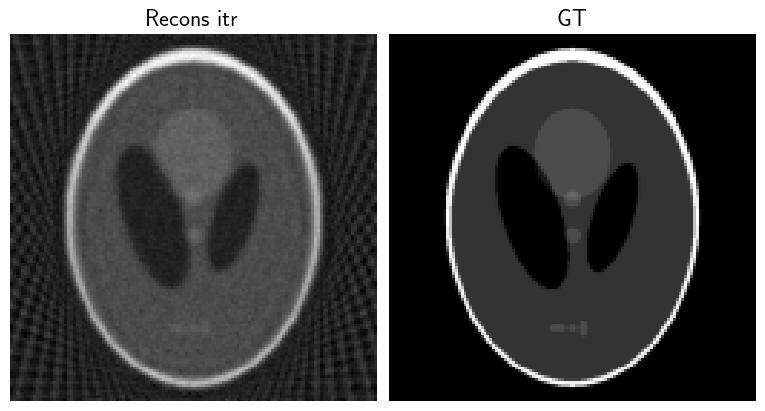
\includegraphics[width=.8\linewidth]{images/gradescent.png}
    \caption{Reconstruction with gradient method results.}
    \label{fig:gradescent}
\end{figure}

\subsubsection{Tikhonov Regularisation}

Penalizing large norms yields the \textit{Tikhonov} problem:
\begin{equation}
    u_\alpha^* = \arg\min_{u} \left\{ \tfrac{1}{2}\|\mathbf{A}u - y\|^2 + \alpha\|u\|^2 \right\}.
\end{equation}

but $u_\alpha^*$ can be found solving a linear system with symmetric, positive definite, matrix.
The first-order optimality condition gives $(\mathbf{A}^\top\mathbf{A} + \alpha I)u_\alpha^* = \mathbf{A}^\top y$, which is solved iteratively by replacing \textit{ZeroPrior} with \textit{dinv.optim.Tikhonov()} and setting \textit{"lambda": 0.1} in \textit{params\_algo}. The rest is similar to listing \ref{code:gd}.

\subsubsection{LASSO / Sparsity-Promoting Regularisation}

The lasso penalizes solutions with large $1$-norms, promoting solutions with few non-zero entries:
\begin{equation}
    u_\alpha^* = \arg\min_{u} \left\{ \tfrac{1}{2}\|\mathbf{A}u - y\|^2 + \alpha\|u\|_1 \right\}.
\end{equation}
This is solved by \textit{Proximal Gradient Descent} (PGD), where the proximal operator of $\alpha\|\cdot\|_1$ is soft-thresholding $S_\alpha(u) = \operatorname{sign}(u)(|u|-\alpha)^+$.

In code, we just have to \textit{iteration="PGD"} and \textit{prior=dinv.optim.L1Prior()}. 

The above algorithms need to be tuned with hyperparameters, for example \textit{step size}. We can visualize how the MSE, PSNR, and SSIM vary with different step sizes for the three algorithms. Results are shown in figure \ref{fig:msepsnrssim}. It is interesting to notice that, with \textit{deepinv} default $\lambda$ value, the zerio-prior algorithm seems to outperform the others.

\begin{figure}[h]
    \centering
    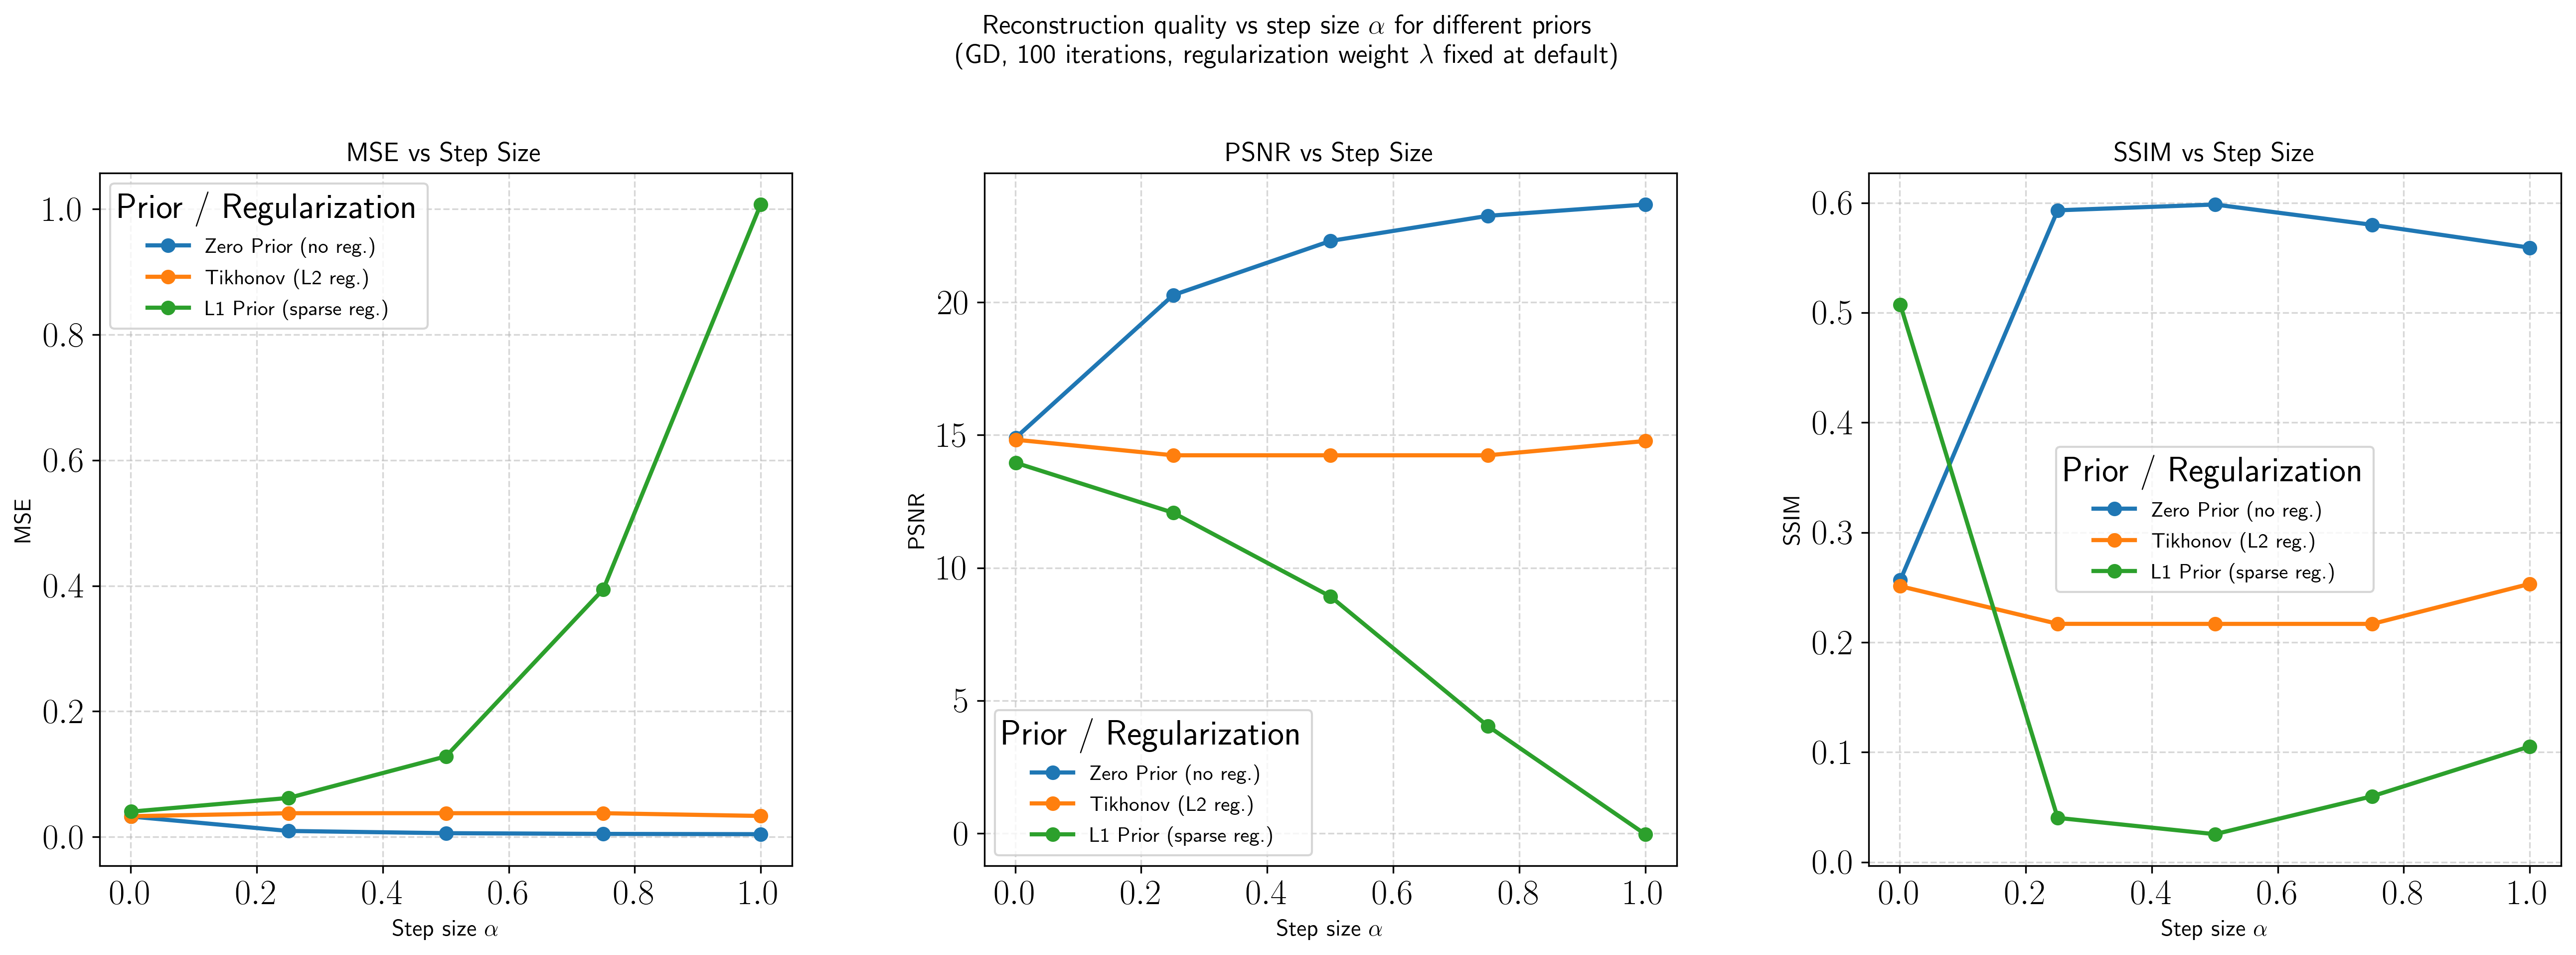
\includegraphics[width=\linewidth]{images/stepsizecompar.png}
    \caption{Hyperparameters comparison: MSE (left), PSNR (center), and SSIM (right).}
    \label{fig:msepsnrssim}
\end{figure}

\subsection{Learned Regularisation Functionals}
TODO

Up until this point we have seen how to solve the inverse problem using model-based reconstruction, by explicitly defining a regularization function that minimizes a cost function. While rigorous, hand-crafted priors are too static to capture complex and nuanced textures.  

We will now try to learn the \textit{regularisation functionals}. Instead of manually defining the regularizer, we will learn the prior distribution implicitly from data.

We will use the same class as before to add Gaussian noise, as well as a similar initialized module physics.


The first step is creating a supervised dataset by constructing $\{(y_i,u_i)\}_{i=1}^N$, where $u_i$ is an image from a dataset, specifically the MNIST datasets, taken from the \textit{datasets} module of the \textit{torchvision} library. We generate a dataset with two sub-datasets, one for training and one for testing, which is standard best practice.
Two samples from the dataset can be seen in figure \ref{fig:samples}.

\begin{figure}[h]
    \centering
    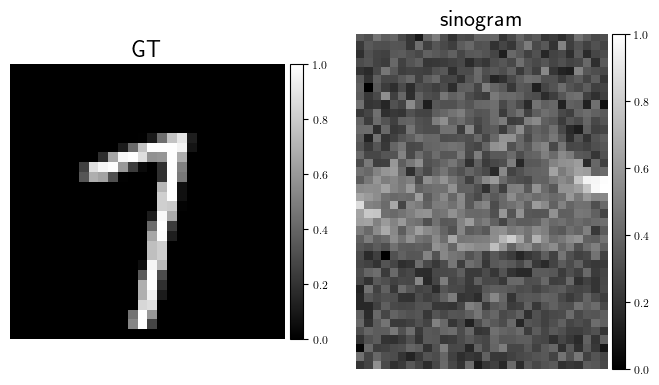
\includegraphics[width=.8\linewidth]{images/samplesdataset.png}
    \caption{Samples from train dataset constructed from MNIST. Ground truth on the left, sinogram on the right.}
    \label{fig:samples}
\end{figure}

First, we compute a reconstruction baseline with an L1 prior, step size of one and a lambda of $0.05$. We run the model builder for five hundred iterations to find and optimal solution. Results can be seen in figure \ref{fig:l1priorbaseline}.

\begin{figure}[h]
    \centering
    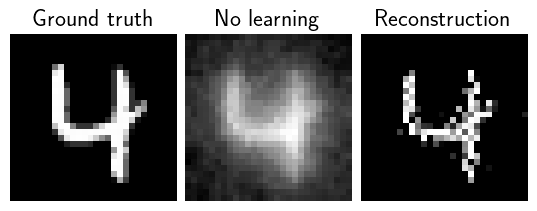
\includegraphics[width=.8\linewidth]{images/baselinel1.png}
    \caption{Baseline reconstruction with L1 prior, step size 1, lambda $0.05$ and 500 iterations.}
    \label{fig:l1priorbaseline}
\end{figure}

\subsection{Plug-and-Play with a Pre-trained Denoiser}

\textit{Plug-and-Play} (PnP) replaces the proximal step in PGD with a pre-trained denoising network $D_{\theta,\sigma}$, obtaining:
\begin{equation}
\left\{
    \begin{aligned}
        z^{(k+1)} &= u^{(k)} - \tau A^\top(Au^{(k)}-y) \\
        u^{(k+1)} &= D_{\theta,\sigma}(z^{(k+1)})
    \end{aligned}
\right.
\end{equation}

Now is the network itself that plays the role of denoiser, in particular it is trained to remove the Gaussian noise.

We first evaluate the results of a \textit{DnCNN} network pre-trained on natural images, directly available from the DeepInverse library of models. An example code is shown in listing \ref{code:dncnn}.

\begin{lstlisting}[language=Python, label={code:dncnn}, caption={PnP-PGD with a pre-trained DnCNN denoiser.}]
from deepinv.models import DnCNN

denoiser = DnCNN(in_channels=1, out_channels=1,
                 pretrained="download", device=device)
prior = PnP(denoiser=denoiser)

modelPnP = optim_builder(
    iteration="PGD",
    prior=prior,
    data_fidelity=dinv.optim.data_fidelity.L2(),
    early_stop=True,
    max_iter=200,
    params_algo={"stepsize": 0.8, "g_param": 0.1}
)
\end{lstlisting}

The resulting reconstruction leaves a lot to be desired, looking even worse than the baseline, as shown in figure \ref{fig:dncnn}.

\begin{figure}[h]
    \centering
    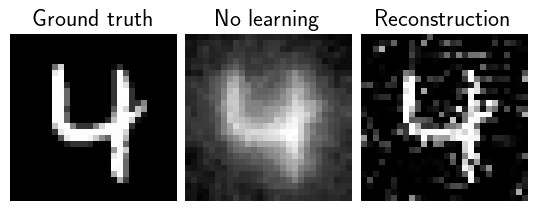
\includegraphics[width=.8\linewidth]{images/dncnndenoiser.png}
    \caption{Reconstruction with DnCNN pretrained on natural images as prior.}
    \label{fig:dncnn}
\end{figure}

\subsection{Training a Task-Specific Denoiser}

Now we want to train a \textit{DnCNN} denoiser specifically on the \textit{MNIST} dataset. 

First we create a new dataset $\{\tilde{u}_i,u_i\}_{i=1}^{N_{den}}$ such that $\tilde{u}_i = u_i + \tilde{\epsilon}_i$ where $\tilde{\epsilon}_i \sim \mathcal{N}(0,\sigma^2 I)$.

Then we define a denoiser $D_\theta$ and train it. We choose its parameters $\theta$ so to minimize
\begin{equation}
    L_{den}(\theta) = \frac{1}{N_{den}} \sum_{i=1}^{N_{den}} \| D_\theta(\tilde{u}_i) - u_i\|^2
\end{equation}

Finally, we use the trained denoiser in any PnP scheme.

Training uses \textit{dinv.Trainer} with the Adam optimiser for 20 epochs. The trained denoiser is then plugged into PnP-PGD and evaluated on the CT test set. An example code for the training can be seen in listing \ref{code:dncnntrain}.

\begin{lstlisting}[language=Python, label={code:dncnntrain}, caption={Training a DnCNN denoiser.}]
denoiser_train = DnCNN(in_channels=1, out_channels=1,
                pretrained="download",device=device,)
noise_model = dinv.physics.GaussianNoise(sigma=sigma_PnP)

trainer_den = dinv.Trainer(
    model=denoiser_train,
    physics=dinv.physics.Denoising(noise_model=noise_model),
    train_dataloader=DataLoader(train_dataset, batch_size=batch_size, num_workers=0, shuffle=False),
    eval_dataloader=DataLoader(test_dataset, batch_size=batch_size, num_workers=0, shuffle=False),
    epochs=20,
    losses=[dinv.loss.SupLoss(metric=dinv.loss.metric.MSE())],
    optimizer=torch.optim.Adam(denoiser_train.parameters(), lr=learning_rate),
    device=device,
)
\end{lstlisting}

Now that we have a trained denoiser, we can use it as prior to evaluate its performances. The results, shown in figure \ref{fig:pnptrained}, are satisfactory: the reconstructed image looks very close to the ground truth, and is a considerable improvement over our previous baseline.

\begin{figure}[h]
    \centering
    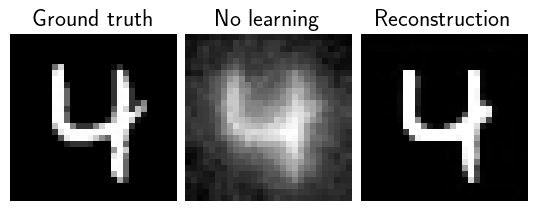
\includegraphics[width=.8\linewidth]{images/pnp_trained.png}
    \caption{Reconstruction with a DnCNN trained for the specific task. The resulting image is remarkably close to the ground truth, and improve significantly over the baseline.}
    \label{fig:pnptrained}
\end{figure}

\subsection{Summary}

The lab progressively builds from analytic inversion (FBP) to variational regularisation (Tikhonov, LASSO, TV) and finally to learned Plug-and-Play priors. Table~\ref{tab:methods} summarises the methods.

\begin{table}[h]
\centering
\caption{Summary of reconstruction methods explored in the lab.}
\label{tab:methods}
\begin{tabular}{lccc}
\hline
\textbf{Method} & \textbf{Algorithm} & \textbf{Prior}  \\
\hline
FBP             & Analytic           & None                 \\
GD (unregul.)   & Gradient Descent   & None                 \\
Tikhonov        & Gradient Descent   & Gaussian            \\
LASSO           & PGD                & Gaussian            \\
PnP (pretrained)& PGD                & Pretrained DnCNN     \\
PnP (trained)   & PGD                & Task-trained DnCNN   \\
\hline
\end{tabular}
\end{table}


\section{Conclusion}

This report has traced a coherent path from physical measurement to high-quality image reconstruction across two distinct but mathematically unified modalities. In both ISM and CT, the core challenge is the same: inverting a compact linear operator whose naïve inversion is unstable, and compensating for incomplete or noisy data through principled regularisation or learned priors.

The practical experiments on CT reconstruction illustrate the strength of machine learning techniques and the importance of domain-specific training. Starting from Filtered Back-Projection, which degrades quickly, through iterative methods with hand-crafted priors, such as Tikhonov and LASSO, we managed to get closer to a satisfactory image reconstruction. To improve the results, we tried to use a pretrained DnCNN denoiser as prior, which yielded worse results compared to the classical methods. We then tried to train the DnCNN denoiser on the dataset itself, thus using a denoiser trained on the specific task, which resulted in a significant improvement in the output..

Taken together, the results reinforce a central insight of modern computational imaging: the forward model provides the physics, but reconstruction quality ultimately depends on how well the prior captures the statistics of the target domain. 
%
%
%\input{sections/socialnetworks}
%
%\input{sections/goal}
%
%\input{sections/corpora}
%
%\input{sections/langanalysis}
%
%\input{sections/sentanalysis}
%
%\section{Conclusion}

This report has traced a coherent path from physical measurement to high-quality image reconstruction across two distinct but mathematically unified modalities. In both ISM and CT, the core challenge is the same: inverting a compact linear operator whose naïve inversion is unstable, and compensating for incomplete or noisy data through principled regularisation or learned priors.

The practical experiments on CT reconstruction illustrate the strength of machine learning techniques and the importance of domain-specific training. Starting from Filtered Back-Projection, which degrades quickly, through iterative methods with hand-crafted priors, such as Tikhonov and LASSO, we managed to get closer to a satisfactory image reconstruction. To improve the results, we tried to use a pretrained DnCNN denoiser as prior, which yielded worse results compared to the classical methods. We then tried to train the DnCNN denoiser on the dataset itself, thus using a denoiser trained on the specific task, which resulted in a significant improvement in the output..

Taken together, the results reinforce a central insight of modern computational imaging: the forward model provides the physics, but reconstruction quality ultimately depends on how well the prior captures the statistics of the target domain. 
%%
%% The acknowledgments section is defined using the "acks" environment
%% (and NOT an unnumbered section). This ensures the proper
%% identification of the section in the article metadata, and the
%% consistent spelling of the heading.
%% \begin{acks}
%% To Robert, for the bagels and explaining CMYK and color spaces.
%% \end{acks}

%%
%% The next two lines define the bibliography style to be used, and
%% the bibliography file.
\bibliographystyle{ACM-Reference-Format}
\bibliography{report}


\end{document}
\endinput
%%
%% End of file `sample-manuscript.tex'.
